\jxhj{%教学后记
	}
\skrq{%授课日期
	2017年11月24 4-5节}
\ktmq{%课题名称
	 Fanuc上的孔加工指令(一)}
\jxmb{%教学目标,每行前面要加 \item
	\item 掌握孔加工的加工工艺;
	\item 掌握Fanuc上的孔加工指令的选用;
	\item 掌握Fanuc上孔加工指令的使用;
	\item 会进行孔加工程序的编写。}
\jxzd{%教学重点,每行前面要加 \item
	\item Fanuc上孔加工指令的使用;
	\item 进行孔加工程序的编写。 }
\jxnd{%教学难点,每行前面要加 \item
	\item 进行孔加工程序的编写。 }
\jjff{%教学方法
	通过讲述、举例、演示法来说明;}

\makeshouye %制作教案首页

%%%%教学内容
\subsection{组织教学}
\begin{enumerate}[\hspace{2em}1、]
	\item 集中学生注意力;
	\item 清查学生人数;
	\item 维持课堂纪律;
\end{enumerate}

\subsection{复习导入及主要内容}
\begin{enumerate}[1、]
\item 孔加工刀具;
\item 孔加工方式;
\item 铣孔与钻孔;
\item 孔加工编程。
\end{enumerate}

\subsection{教学内容及过程}
\subsubsection{孔加工固定循环指令}
为了简化编程,节省存储空间,把孔加工过程做成固定循环,存储在CNC系统中。Fanuc上的固定循环有G73、G74、G76、G81-G89,其指令格式如下:

\[ 
\left\lbrace 
\begin{array}{c}
G90 \\ G91
\end{array} 
\right\rbrace 
\left\lbrace 
\begin{array}{c}
G99 \\ G98
\end{array} 
\right\rbrace  
 G\_ X\_ Y\_ Z\_ R\_ Q\_ K\_ F\_    \]

说明:

(1)G90/G91:绝对值与增量值,如图11-2,左G90,右G91

(2)G98/G99:返回平面选择

G98返回初始平面

G99返回R点平面

(3)G:孔加工方式

(4)X、Y:孔加工的位置

(5)Z:孔底平面的位置(G91时是R点到孔底的增量值)

(6)R:R点平面的位置(G91时是初始平面到孔
R点平面的增量值,G90时是R点平面Z向绝对坐标)

(7)参数Q:G73、G74深孔中每次Z向进刀量,G76、G87镗孔中的偏移量

(8)参数P:有孔底暂停的暂停时间

(9)参数F:孔加工中的切削速度

(10)参数K、L:固定循环重复次数,结合G91功能更大。

\begin{figure}[h]
	\centering
	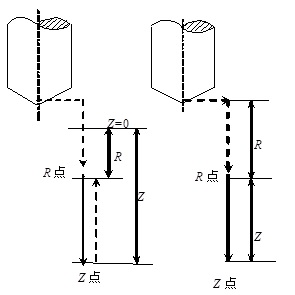
\includegraphics[width=0.7\linewidth]{data/image/21-1}
	\caption{孔加式中的G90与G91}
	\label{fig:21-1}
\end{figure}

注意:孔加工固定循环指令为模态指令,要用G80或01组的指令取消。孔加工参数(重复次数KL除外)也是模态的,在被改变和取消之前一直保持,即使是孔加工方式被改变,也保持。



\subsubsection{孔加工方式其参数}
G81 X\_ Y\_ Z\_ R\_ F\_;用于浅孔,中心孔

G82 X\_ Y\_ Z\_ R\_ P\_ F\_;用于钻孔、锪孔等 

G73 X\_ Y\_ Z\_ R\_ Q\_ F\_;用于深孔(把深孔当作几个浅孔)

G85 X\_ Y\_ Z\_ R\_ F\_;用于铰孔(与G81不同的是慢速提刀)

G84 X\_ Y\_ Z\_ R\_ P\_ F\_;用于右螺纹攻丝

其它:

G74 X\_ Y\_ Z\_ R\_ P\_ F\_;用于左螺纹攻丝

G76 X\_ Y\_ Z\_ R\_ P\_ Q\_ F\_;用于精镗孔

G83 X\_ Y\_ Z\_ R\_ Q\_ F\_;用于深孔、小孔(可排屑)

G86 X\_ Y\_ Z\_ R\_ F\_;用于镗孔(孔底主轴停)

G87 X\_ Y\_ Z\_ R\_ P\_ Q\_ F\_;反向镗孔

G86 X\_ Y\_ Z\_ R\_ F\_;有手动返回的镗孔

G89 X\_ Y\_ Z\_ R\_ P\_ F\_;镗孔(与G85不同的是有孔底暂停)


\subsubsection{加工实例}

加工如\ref{fig:21-2}所示的零件,其中孔的有效深度为30mm。

\begin{figure}
	\centering
	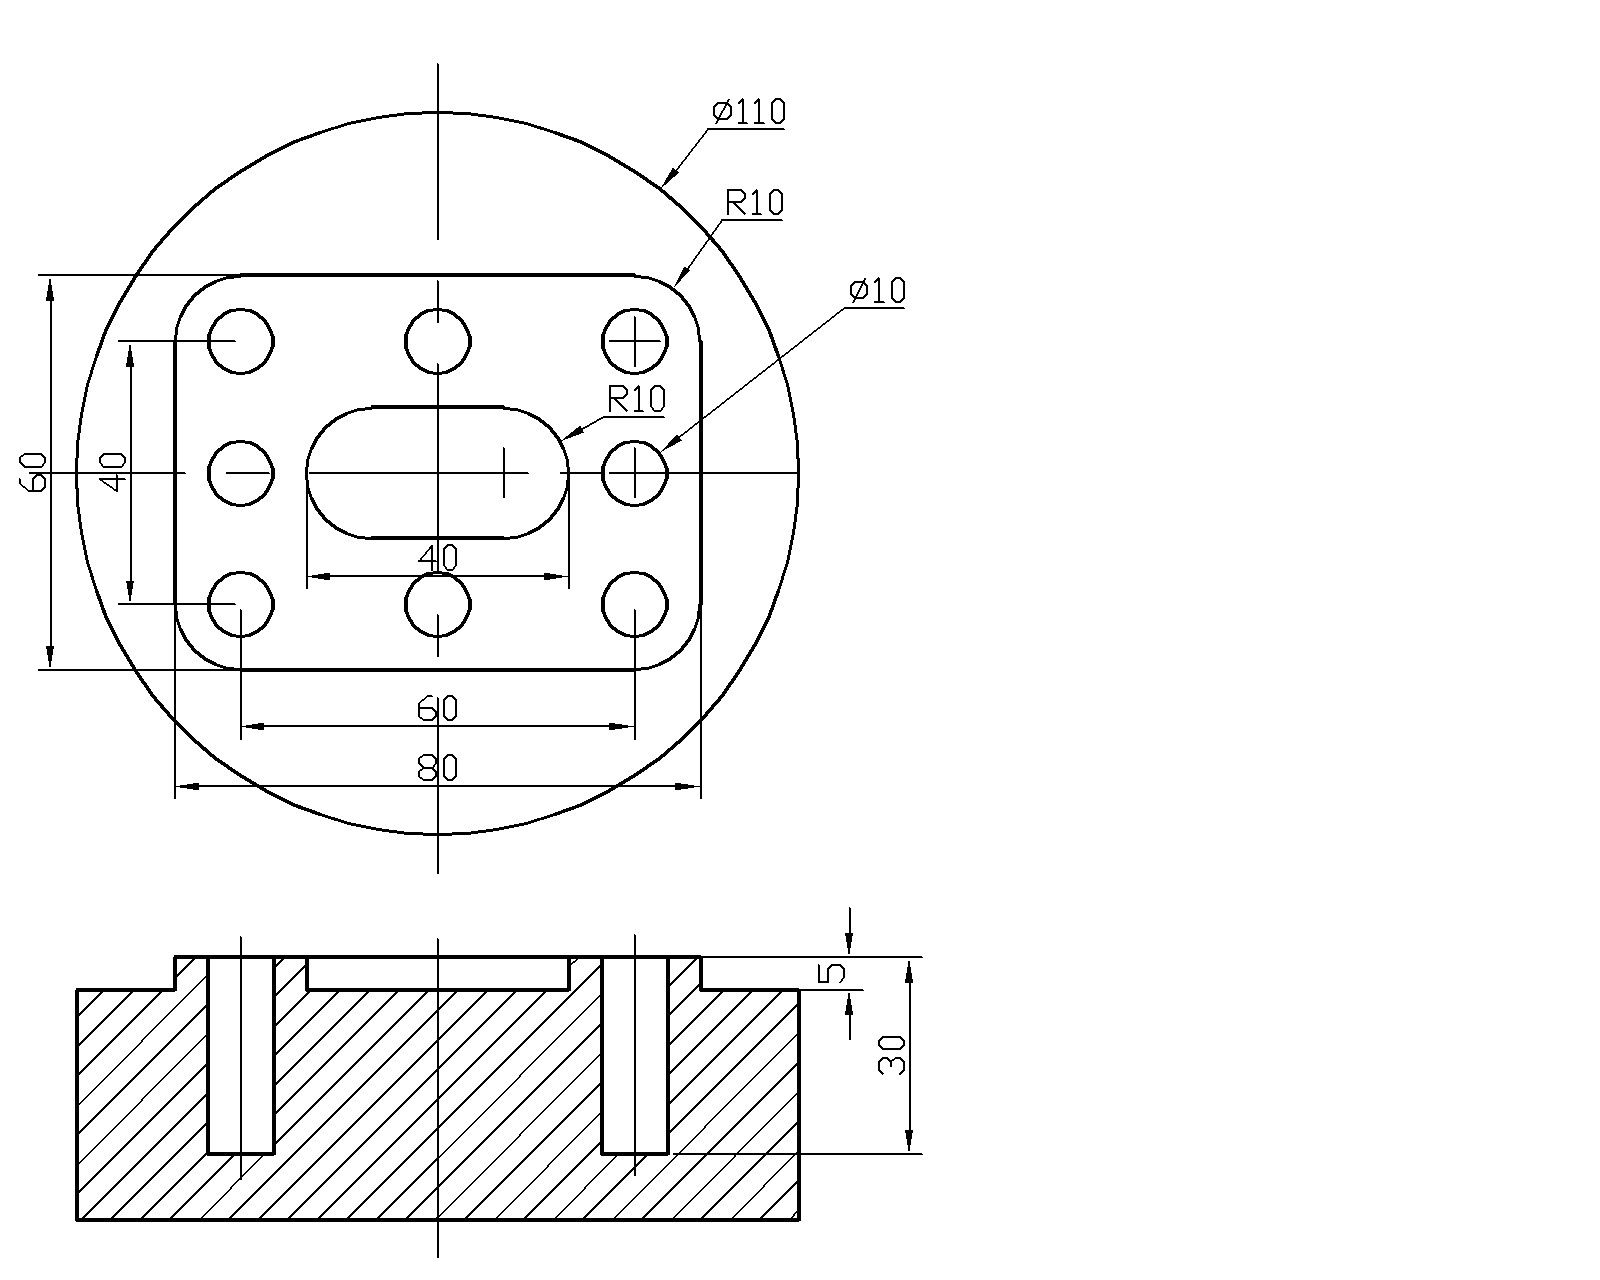
\includegraphics[width=0.5\linewidth,trim=0 0 450  0,clip]{data/image/21-2}
	\caption{孔加工实例}
	\label{fig:21-2}
\end{figure}

1、孔加工方法:钻中心孔、钻孔、铰孔

2、刀具:

$\varnothing $3中心钻(切削刃长10mm,加工深度6-8mm,粗对刀即可)S1200 F120 Z-6.0

$\varnothing $9.8麻花钻 S550 F80.0 Z-35.0 (比32多3mm)

$\varnothing $10机用铰刀 S300 F50 Z-32.0 (比30多2mm)

4、参考程序:
\begin{lstlisting}

O0001;(钻中心孔)
G54 G17 G40 G49 G90;
M3 S1200;
G0 Z30.0;
G99 G81 X-30.0 Y-20.0 Z-6.0 R5.0 F120;
X0
X30.0
Y0
X0
X-30.0
Y20.0
X0
G98 X30.0
M5
M30

\end{lstlisting}

\begin{lstlisting}

O0001;(钻孔)
G55 G17 G40 G49 G90;
M3 S500;
G0 Z30.0;
G99 G83 X-30.0 Y-20.0 Z-6.0 R5.0 Q5.0 F60;
X0
X30.0
Y0
X0
X-30.0
Y20.0
X0
G98 X30.0
M5
M30
\end{lstlisting}


\subsection{课堂小结}
\begin{enumerate}[1、]
\item Fanuc孔加工指令;
\item Fanuc 孔加工应用;
\item Fanuc 孔加工编程;
\item 编程实例。
\end{enumerate}

\vfill
\subsection{布置作业}
\begin{enumerate}[1、]
	\item 综合习题一。
\end{enumerate}
\vfill